\documentclass{beamer}
\usepackage{amsfonts,amsmath,oldgerm}
\usepackage{lmodern}
\usepackage[T1]{fontenc}
\usetheme{sintef}

\newcommand{\testcolor}[1]{\colorbox{#1}{\textcolor{#1}{test}}~\texttt{#1}}

\usefonttheme[onlymath]{serif}

\titlebackground*{assets/background}

\newcommand{\hrefcol}[2]{\textcolor{cyan}{\href{#1}{#2}}}

\title{Design and development of beaconing protocols for smart buoys}
\subtitle{A Custom Simulator for Infrastructure Free Wi-Fi Safety Networks}
\course{Master's Degree in Computer Science}
\author{{Cesare Corsi}}
\IDnumber{2156214}
\date{Academic Year 2024/2025}

\begin{document}
\maketitle

\section{Introduction}

\begin{frame}{Context and Motivation}
\textbf{The Safety Gap:}
\begin{itemize}
\item Large ships: AIS, radar systems for navigation
\item \alert{Small craft, swimmers, divers lack proximity awareness}
\item Traditional systems designed for large scale ship to ship communication
\end{itemize}

\vspace{0.3cm}
\textbf{Existing Solutions Fall Short:}
\begin{itemize}
\item \textbf{AIS}: Expensive, power hungry, requires licensing
\item \textbf{Cellular tracking}: Needs infrastructure, unstable coverage
\item \textbf{Emergency beacons}: Emergency only, no continuous proximity awareness
\end{itemize}

\vspace{0.3cm}
\begin{block}{Critical Need}
Infrastructure free, distributed, low cost proximity detection for coastal safety
\end{block}
\end{frame}

\begin{frame}{Wi-Fi Beaconing: Promising Yet Challenging}
\begin{columns}
\begin{column}{0.58\textwidth}
\textbf{Why Wi-Fi?}
\begin{itemize}
\item Present in modern smartphones/wearables
\item Infrastructure free broadcast capability
\item 100-300m range suitable for coastal proximity
\item Low cost
\end{itemize}

\vspace{0.3cm}
\textbf{The Scalability Challenge:}
\begin{itemize}
\item IEEE 802.11 DCF: \alert{fixed parameters}
\item CSMA/CA with predefined backoff
\item High density $\Rightarrow$ collision probability increases
\item \alert{Reliability degradation unacceptable for safety}
\end{itemize}
\end{column}
\begin{column}{0.38\textwidth}
\begin{center}
\vspace{0.3cm}
\textit{Periodic beacon broadcasts announce presence}

\vspace{0.8cm}
\textbf{More Nodes}\\$\Downarrow$\\
\textbf{More Collisions}\\$\Downarrow$\\
\textbf{Lost Beacons}\\$\Downarrow$\\
\alert{\textbf{Safety Risk}}
\end{center}
\end{column}
\end{columns}
\end{frame}

\begin{frame}{Research Questions}
\begin{enumerate}
\item How does \textbf{node density} affect reliability in infrastructure free broadcast networks?

\vspace{0.4cm}
\item Can \textbf{straightforward local adaptation} mechanisms improve scalability without requiring global coordination or infrastructure?

\vspace{0.4cm}
\item How to develop a reliable \textbf{simulator} that realistically reflects MAC layer broadcast behavior for evaluating adaptive protocols?
\end{enumerate}
\end{frame}

\begin{frame}{Thesis Contributions}
\textbf{Primary Contribution:}\\
\vspace{0.2cm}
Custom discrete event simulator for evaluating broadcast protocols in infrastructure free wireless networks

\vspace{0.5cm}
\textbf{Case Study:}\\
\vspace{0.2cm}
ProSafe, proximity safety system with ADAB (Adaptive Density Aware Beaconing) protocol
\end{frame}

\section{ProSafe System}

\begin{frame}{ProSafe: Proximity-based Safety Network}
\textbf{Minimalist Wi-Fi System for Maritime Proximity Detection}

\vspace{0.3cm}
\begin{columns}
\begin{column}{0.55\textwidth}
\begin{itemize}
    \item \textbf{Infrastructure free:} No APs, routers, or internet required
    \item \textbf{Pure broadcast:} MAC layer only, no IP protocols
\end{itemize}
\end{column}
\begin{column}{0.45\textwidth}
\begin{itemize}
    \item \textbf{Passive vessels:} Boats passive listen to nearby buoys
    \item \textbf{Energy efficient and low cost:} Simple hardware
\end{itemize}
\end{column}
\end{columns}

\vspace{0.3cm}
\begin{center}
\includegraphics[width=0.5\textwidth]{../thesis/img/system.png}
\end{center}
\end{frame}

\begin{frame}{Beacon Structure and Discovery}
\textbf{Broadcast frames to FF:FF:FF:FF:FF:FF ($\sim$500 bytes):}
\begin{itemize}
\item \textbf{Buoy ID:} UUID (16 bytes)
\item \textbf{Timestamp:} Transmission time (4 bytes)
\item \textbf{Position:} GPS coordinates (8 bytes)
\item \textbf{Neighbor list:} Recently heard neighbors (28 bytes each)
    \begin{itemize}
    \item UUID, timestamp, position per neighbor
    \item \alert{Dynamic length grows with local density}
    \end{itemize}
\end{itemize}

\vspace{0.3cm}
\begin{block}{Indirect Discovery}
When buoy A receives beacon from B containing C in neighbor list, A learns about C without direct reception $\Rightarrow$ \textbf{Extended awareness}
\end{block}
\end{frame}

\begin{frame}{MAC Layer: IEEE 802.11 DCF}
\begin{columns}[t]
\begin{column}{0.55\textwidth}
\textbf{CSMA/CA Mechanism:}
\begin{enumerate}
\item Sense channel
\item If busy, wait
\item If idle for DIFS ($50 \mu s$)
\item Start backoff timer $[0, \text{CW}]\times \text{slot time}$
\begin{itemize}
    \item If the channel is idle, decrement the backoff counter
    \item If the channel is busy, freeze the backoff counter
\end{itemize}
\item When backoff reaches zero, transmit
\end{enumerate}
\end{column}

\begin{column}{0.42\textwidth}
\textbf{Broadcast Limitations:}
\begin{itemize}
\item \alert{No ACKs} $\Rightarrow$ no delivery feedback
\item \alert{No RTS/CTS} $\Rightarrow$ hidden terminal
\item \alert{Silent failures} $\Rightarrow$ undetected collisions
\end{itemize}
\vspace{0.3cm}
$\Rightarrow$ \textbf{Adaptive mechanisms needed without explicit feedback}
\end{column}
\end{columns}

\end{frame}

\section{ADAB Protocol}

\begin{frame}{Static Beaconing Protocol (SBP) - Baseline}
\textbf{Simple but Non Scalable Approach:}
\begin{itemize}
\item Fixed beacon interval: $BI_{\text{static}} = 0.25$ s
\item \alert{All nodes transmit at same rate regardless of density}
\end{itemize}

\vspace{0.3cm}
\begin{columns}[t]
\begin{column}{0.48\textwidth}
\textbf{Sparse (low density):}
\begin{itemize}
\item Works well
\item Low collision probability
\end{itemize}
\end{column}
\begin{column}{0.48\textwidth}
\textbf{Dense (high density):}
\begin{itemize}
\item Channel overload
\item More collisions
\item Wasted energy
\end{itemize}
\end{column}
\end{columns}

\vspace{0.4cm}
$\Rightarrow$ \textbf{Fixed parameters cannot adapt to varying conditions}
\end{frame}

\begin{frame}{ADAB: Adaptive Density-Aware Beaconing}

\vspace{0.3cm}
\textbf{Design:}
\begin{itemize}
\item \textbf{Sparse scenarios:} Few neighbors $\Rightarrow$ beacon frequently for rapid discovery
\item \textbf{Dense scenarios:} Many neighbors $\Rightarrow$ reduce rate to lower collisions
\item \textbf{Local only:} Uses neighbor count, no global coordination
\end{itemize}

\vspace{0.3cm}
\textbf{Formula:}
$$
BI = BI_{\text{min}} + \left(\min\left\{\cfrac{N}{N_{\text{thr}}}, 1.0\right\}\right)^2 \times (BI_{\text{max}} - BI_{\text{min}})
$$
\end{frame}

\begin{frame}{ADAB: Energy Consumption Estimation}
\textbf{Transmission energy calculation:}
\begin{itemize}
\item Airtime: 4.4 ms (500 bytes at 1 Mbps + overhead)
\item Power: $P_{\text{TX}} \approx 1$ W
\item Per beacon: $E_{\text{beacon}} = 4.4$ mJ
\end{itemize}

\vspace{0.3cm}
\textbf{Hourly consumption vs. neighbor count:}
\begin{center}
\begin{tabular}{cccc}
\hline
\textbf{Neighbors} & \textbf{Interval} & \textbf{Energy (J/h)} & \textbf{Savings} \\
\hline
0 (sparse) & 0.25 s & 63.4 & -- \\
3 & 0.44 s & 36.0 & 43\% \\
7 & 1.28 s & 12.4 & 81\% \\
$\geq$10 (dense) & $\geq$2.36 s & $\leq$6.7 & $\geq$89\% \\
\hline
\end{tabular}
\end{center}

\vspace{0.3cm}
\textbf{Dual benefit:} Longer intervals $\Rightarrow$ \alert{both} lower energy \alert{and} reduced collisions
\end{frame}

\section{Simulator}

\begin{frame}{Simulator Architecture}
\textbf{Why Custom Simulator?}
\begin{itemize}
\item General purpose tools (ns-3, OMNeT++) complex and time consuming
\item \alert{Full control} over implementation details
\item \alert{Simplicity:} Only components needed for research
\item Easy modification and extension
\end{itemize}

\vspace{0.3cm}
\textbf{Discrete Event Simulation:}
\begin{itemize}
\item Priority queue for time ordered processing
\item \textbf{12 event types:} Scheduler checks, channel sensing, DIFS, backoff, TX start/end, reception, neighbor cleanup, movement, etc.
\end{itemize}
\end{frame}

\begin{frame}{Simulator State Diagram}
\begin{center}
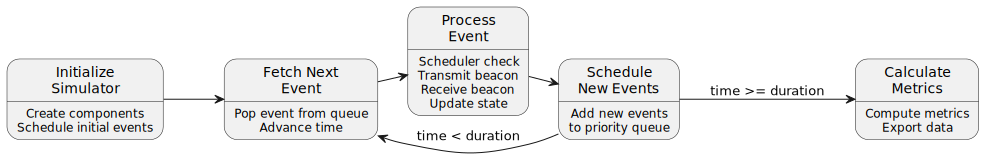
\includegraphics[width=\textwidth]{../thesis/img/uml_state.png}
\end{center}
\end{frame}

\begin{frame}{Channel Model: Calibrated from Sea Trials}
\textbf{Field measurement setup:}
\begin{itemize}
\item Raspberry Pi 4 + AR9271 USB Wi-Fi adapter
\item Omnidirectional antenna
\item GPS tracking
\end{itemize}

\vspace{0.3cm}
\begin{columns}[t]
\begin{column}{0.3\textwidth}
\textbf{Measured reception rates:}
\begin{center}
\begin{tabular}{cc}
\hline
\textbf{Distance} & \textbf{$P_{\text{rx}}$} \\
\hline
0-70 m & $\sim$0.9 \\
70-120 m & $\sim$0.15 \\
$>$ 120 m & $\sim$0.0 \\
\hline
\end{tabular}
\end{center}
\end{column}
\begin{column}{0.3\textwidth}
\textbf{Two channel modes:}
\begin{itemize}
\item \textbf{Ideal:} Isolate MAC effects
\item \textbf{Probabilistic:} Realistic propagation
\end{itemize}
\end{column}
\begin{column}{0.3\textwidth}
\textbf{Collision detection:}
\begin{itemize}
\item Detect temporal and spatial overlap
\item Models hidden terminal problem
\end{itemize}
\end{column}
\end{columns}

\end{frame}

\section{Experimental Results}

\begin{frame}{Experimental Setup}
\textbf{Simulation configuration:}
\begin{itemize}
\item 800 $\times$ 800 m area, 20-300 nodes
\item 600 seconds duration, 15 runs per scenario
\item \textbf{Stochastic churn:} Dynamic arrivals/departures every 15-20s
\item 20\% mobile nodes with random velocities
\end{itemize}

\vspace{0.3cm}
\textbf{Key metric - Broadcast Packet Delivery Ratio (B-PDR):}
$$\text{B-PDR} = \frac{\sum_{i=1}^{N_{\text{tx}}} n_{\text{rcv},i}}{\sum_{i=1}^{N_{\text{tx}}} n_{\text{intended},i}}$$

\vspace{0.2cm}
\begin{itemize}
\item Fraction of intended beacon receptions that succeed
\item \alert{Fundamental reliability requirement for safety systems}
\end{itemize}
\end{frame}

\begin{frame}{Results: B-PDR vs Node Population (Ideal Channel)}
\begin{columns}
\begin{column}{0.55\textwidth}
\includegraphics[width=\textwidth]{../thesis/img/bpdr_ideal.png}
\end{column}
\begin{column}{0.42\textwidth}
\textbf{Findings:}
\begin{itemize}
\item \textbf{SBP:} Monotonic decline\\0.95 $\to$ 0.70 (25\% loss)
\item \textbf{ADAB:} Constant\\0.97-0.98 across range
\item Neighbors: $\sim$3 $\to$ $\sim$19
\end{itemize}

\vspace{0.3cm}
\begin{block}{Insight}
Local contention drives SBP degradation; ADAB adapts successfully
\end{block}
\end{column}
\end{columns}
\end{frame}

%\begin{frame}{Results: Collision Rate Explains Reliability}
%\begin{columns}
%\begin{column}{0.45\textwidth}
%\textbf{Collision rate trend:}
%\begin{itemize}
%\item \textbf{SBP:} Linear increase\\2\% $\to$ 31\% (one in three beacons collide)
%\item \textbf{ADAB:} Flat $<$ 4\%\\despite density growth
%\end{itemize}
%
%\vspace{0.3cm}
%\begin{block}{Causal Relationship}
%SBP's rising collisions $\Rightarrow$ B-PDR degradation\\
%ADAB's stable collisions $\Rightarrow$ consistent reliability
%\end{block}
%\end{column}
%\begin{column}{0.5\textwidth}
%\includegraphics[width=\textwidth]{../thesis/img/collision_rate.png}
%\end{column}
%\end{columns}
%\end{frame}

\begin{frame}{Results: Probabilistic Channel (Realistic Conditions)}
\begin{columns}
\begin{column}{0.45\textwidth}
\textbf{Dual loss sources:}
\begin{itemize}
\item \alert{Collisions} (MAC layer)
\item \alert{Distance based failures} (physical layer)
\end{itemize}

\vspace{0.3cm}
\textbf{Performance realistic conditions:}
\begin{itemize}
\item \textbf{SBP:} 0.39 $\to$ 0.30 (further degradation)
\item \textbf{ADAB:} 0.40-0.42 (stable)
\end{itemize}

\end{column}
\begin{column}{0.5\textwidth}
\includegraphics[width=\textwidth]{../thesis/img/bpdr_non_ideal.png}
\end{column}
\end{columns}
\end{frame}

\section{Conclusions}

\begin{frame}{Limitations}
\textbf{Deliberate simplifications focused on MAC layer research:}

\vspace{0.3cm}
\begin{columns}[t]
\begin{column}{0.48\textwidth}
\textbf{Physical Layer:}
\begin{itemize}
\item Constant distance based model
\item No capture effect (all collisions fail)
\item Fixed 1 Mbps PHY rate
\end{itemize}
\end{column}
\begin{column}{0.48\textwidth}
\textbf{Energy:}
\begin{itemize}
\item Not yet modeled inside the simulator
\end{itemize}
\end{column}
\end{columns}

\vspace{0.3cm}
\begin{columns}[t]
\begin{column}{0.48\textwidth}
\textbf{Mobility:}
\begin{itemize}
\item Simple kinematic model
\item No currents, tides, wave action
\item Random movement only
\end{itemize}
\end{column}
\begin{column}{0.48\textwidth}
\textbf{Scale:}
\begin{itemize}
\item Tested up to 300 nodes
\item Scenario with bigger vessels is yet to be evaluated
\end{itemize}
\end{column}
\end{columns}

\end{frame}

\begin{frame}{Future Directions}
\begin{columns}[t]
\begin{column}{0.48\textwidth}
\textbf{Enhanced Realism:}
\begin{itemize}
\item \textbf{Packet length dependent loss}
\item \textbf{Capture effect:} Decode stronger signal during collision
\item \textbf{Introducing complex mobility models}
\end{itemize}
\end{column}
\begin{column}{0.48\textwidth}
\textbf{Protocol Extensions:}
\begin{itemize}
\item \textbf{ACAB evaluation:} Multi factor (density + contact recency + mobility)
\item \textbf{Multi hop modes:} Append (passive list sharing) vs Forward (active relay)
\end{itemize}
\end{column}
\end{columns}
\end{frame}

\begin{frame}{Multi Hop Preliminary Results (Normal mode)}
\textbf{Normal mode:} No multi hop, only direct receptions
\begin{center}
\includegraphics[width=0.7\textwidth]{../thesis/img/discovered_none.png}
\end{center}
\end{frame}

\begin{frame}{Multi Hop Preliminary Results (Forward mode)}
\textbf{Forward mode:} Multi hop with active relay, (\alert{1 hop})
\begin{center}
\includegraphics[width=0.7\textwidth]{../thesis/img/discovered_forward.png}
\end{center}
\end{frame}

\begin{frame}{Multi Hop Preliminary Results (Append mode)}
\textbf{Append mode:} Multi hop with passive list sharing
\begin{center}
\includegraphics[width=0.7\textwidth]{../thesis/img/discovered_append.png}
\end{center}
\end{frame}

\begin{frame}{Final Remarks}
\textbf{The thesis contributions:}

\begin{itemize}
\item A reusable simulator platform for protocol research
\item Developing and validation of ADAB protocol and ProSafe system
\item Providing insights into broadcast systems' scalability and adaptation
\end{itemize}
\vspace{0.4cm}
\alert{Simplicity is powerful:} MAC layer broadcast scalability can be significantly improved through straightforward local adaptation with no global coordination, complex measurements, or cross layer optimization involved.

\end{frame}

\backmatter[notitle]

\end{document}